% In this file you should put the actual content of the blueprint.
% It will be used both by the web and the print version.
% It should *not* include the \begin{document}
%
% If you want to split the blueprint content into several files then
% the current file can be a simple sequence of \input. Otherwise It
% can start with a \section or \chapter for instance.

\section{関連するファイルたち}
このpdfで参照しているコマンドがあるMathlibファイルを以下に示す：
\begin{itemize}
  \item {\color{orange} \texttt{Mathlib.LinearAlgebra.Reflection}}: reflectionsの定義など．
  \item {\color{orange} \texttt{Mathlib.LinearAlgebra.RootSystem.Defs}}: RootPairingの定義など．
  \item {\color{orange} \texttt{Mathlib.LinearAlgebra.RootSystem.Reduced}}: RootSystemがReduced (自身と並行なものは$\pm$倍のみ)であることの定義など．
  \item {\color{orange} \texttt{Mathlib.LinearAlgebra.RootSystem.IsValuedIn}}: 任意のRootPairingのpairing ($= 2 \inner{\alpha}{\beta} / \inner{\alpha}{\alpha} = c(\alpha, \beta)$)の取りうる値に関するファイル．特にcrystallographicやCoxeter weightの定義がある．
  \item {\color{orange} \texttt{Mathlib.LinearAlgebra.RootSystem.Finite.Lemmas}}: Coxeter weightの取りうる値など．
  \item {\color{orange} \texttt{Mathlib.LinearAlgebra.RootSystem.CartanMatrix}}: Cartan matrixの定義など．
\end{itemize}

このpdfでは参照していないが，関連する概念があるMathlibファイルを以下に示す：
\begin{itemize}
  \item {\color{orange} \texttt{Mathlib.Analysis.InnerProductSpace.Projection.Basic}}: projectionの定義など．次のreflectionの定義で使う．
  \item {\color{orange} \texttt{Mathlib.Analysis.InnerProductSpace.Projection.Reflection}}: projectionを使ったreflectionの定義など．このpdfで用いたreflectionの定義より具体的である．
  \item {\color{orange} \texttt{Mathlib.GroupTheory.Coxeter.Matrix}}: Coxeter matrixの定義など．$A_n, B_n, \ldots, E_8, I_2(m), H_3, H_4$型に対応するCoxeter matrixも定義されている．
  \item {\color{orange} \texttt{Mathlib.GroupTheory.Coxeter.Basic}}: Coxeter groupやCoxeter systemの定義など．
\end{itemize}

\newpage
\section{数学的な話}
\subsection{Reflections}
$V$を$\R^n$のsubspaceとし，$\alpha, \beta \in V$の標準内積を$\inner{\alpha}{\beta}$と書き，$\alpha$のノルムを$\norm{\alpha} = \sqrt{\inner{\alpha}{\alpha}}$と書く．

\begin{definition}
  $f : \map{V}{V}$を線型写像とする．
  このとき，$f$が\textbf{直交変換}であるとは，
  \begin{equation}
    \inner{f(\alpha)}{f(\beta)} = \inner{\alpha}{\beta}
  \end{equation}
  が成り立つことである．
  また，$V$上の直交変換全体の集合を$O(V)$と書く．
\end{definition}

\begin{definition}
  $\alpha \in V \setminus \{0\}$とする．このとき，
  \begin{equation}
    H_\alpha := \set{\lambda \in V}{\inner{\alpha}{\lambda} = 0} = (\R \alpha)^{\perp}
  \end{equation}
  を$\alpha$に垂直な\textbf{超平面(hyperplane)}という．
\end{definition}

\begin{definition}
  線型写像$s_\alpha : \map{V}{V}$が次を満たすとき，$s_\alpha$を$\alpha$に関する\textbf{鏡映(reflection)}といい，$\alpha$に垂直なhyperplane $H_\alpha$を$s_\alpha$の\textbf{超平面(reflecting hyperplane)}という：
  \begin{enumerate}[label=(\roman*)]
    \item $s_\alpha (\alpha) = -\alpha$, \label{def:ref_self}
    \item $\lambda \in H_\alpha \implies s_\alpha(\lambda) = \lambda$. \label{def:ref_orthogonal}
  \end{enumerate}
\end{definition}

\begin{remark}
  \ref{def:ref_self}, \ref{def:ref_orthogonal}で$s_\alpha$は定まる．
\end{remark}

\begin{proof}
  $\norm{\alpha} = 1$としてよい．
  $\{\alpha, \lambda_1, \ldots, \lambda_m\}$を$V$の正規直交基底とする．
  特に，$\lambda_1, \ldots, \lambda_m \in H_\alpha$である．
  \ref{def:ref_self}, \ref{def:ref_orthogonal}より，これらの行き先はすべて定まるから，$s_\alpha$は定まる．
\end{proof}

\begin{proposition}
  reflectionは次のように表せる：
  \begin{equation}
    s_\alpha (\lambda) = \lambda - 2\frac{\inner{\alpha}{\lambda}}{\inner{\alpha}{\alpha}} \alpha.
  \end{equation}
\end{proposition}

\begin{proof}
  \ref{def:ref_self}を確かめる：
  \begin{equation}
    \alpha - 2 \frac{\inner{\alpha}{\alpha}}{\inner{\alpha}{\alpha}} \alpha
    = \alpha - 2\alpha
    = -\alpha.
  \end{equation}
  \ref{def:ref_orthogonal}を確かめる．$\lambda \in H_\alpha$とすると，$\inner{\alpha}{\lambda} = 0$であるから，
  \begin{equation}
    \lambda - 2\frac{\inner{\alpha}{\lambda}}{\inner{\alpha}{\alpha}} \alpha
    = \lambda - 2 \cdot 0 \cdot \alpha
    = \lambda.
  \end{equation}
\end{proof}

\begin{proposition}
  $s_\alpha$は$V$の直交変換，すなわち$s_\alpha \in O(V)$である．
\end{proposition}

\begin{proof}
  $\lambda, \mu \in V$とし，$\lambda = c_\lambda \alpha + \beta_\lambda,\ \mu = c_\mu \alpha + \beta_\mu$とする($\beta_\lambda, \beta_\mu \in H_\alpha$)．
  このとき，
  \begin{align}
    \inner{s_\alpha(\lambda)}{s_\alpha(\mu)}
    &= \inner{s_\alpha(c_\lambda \alpha + \beta_\lambda)}{s_\alpha(c_\mu \alpha + \beta_\mu)}\\
    &= \inner{-c_\lambda \alpha + \beta_\lambda}{-c_\mu \alpha + \beta_\mu}\\
    &= c_\lambda c_\mu \inner{\alpha}{\alpha} - c_\lambda \inner{\alpha}{\beta_\mu} - c_\mu \inner{\beta_\lambda}{\alpha} + \inner{\beta_\lambda}{\beta_\mu}\\
    &= c_\lambda c_\mu \inner{\alpha}{\alpha} + \inner{\beta_\lambda}{\beta_\mu}.
  \end{align}
  一方，
  \begin{align}
    \inner{\lambda}{\mu}
    &= \inner{c_\lambda \alpha + \beta_\lambda}{c_\mu \alpha + \beta_\mu}\\
    &= c_\lambda c_\mu \inner{\alpha}{\alpha} + c_\lambda \inner{\alpha}{\beta_\mu} + c_\mu \inner{\alpha}{\beta_\lambda} + \inner{\beta_\lambda}{\beta_\mu}\\
    &= c_\lambda c_\mu \inner{\alpha}{\alpha} + \inner{\beta_\lambda}{\beta_\mu}.
  \end{align}
  よって，$\inner{s_\alpha(\lambda)}{s_\alpha(\mu)} = \inner{\lambda}{\mu}$が成り立つから，$s_\alpha \in O(V)$がわかった．
\end{proof}

\begin{lemma} \label{lem:orth_ref_orthinv}
  \label{lem:ref_inner_hold2}
  $t \in O(V)$とする．このとき，$t s_\alpha t^{-1} = s_{t(\alpha)}$が成り立つ．
\end{lemma}

\begin{proof}
  \ref{def:ref_self}を確かめる：
  \begin{equation}
    (t s_\alpha t^{-1})(t(\alpha))
    = (t s_\alpha)(\alpha)
    = t(-\alpha)
    = -t(\alpha).
  \end{equation}
  \ref{def:ref_orthogonal}を確かめる．
  $\lambda \in H_{t(\alpha)}$とすると，$0 = \inner{\lambda}{t(\alpha)} = \inner{t^{-1}(\lambda)}{\alpha}$ i.e., $t^{-1}(\lambda) \in H_\alpha$であるから，
  \begin{equation}
    (t s_\alpha t^{-1})(\lambda)
    = t (s_\alpha(t^{-1}(\lambda)))
    = t(t^{-1}(\lambda))
    = \lambda.
  \end{equation}
\end{proof}

\subsection{Reflection groupsとroot systems}
\begin{definition}
  $O(V)$の部分群$W$が次を満たすとき，$W$を\textbf{有限鏡映群(finite reflection group)}という：
  \begin{enumerate}[label=(\roman*)]
    \item $W$はfinite group,
    \item $W$はreflectionsで生成される，すなわち
    \begin{equation}
      \forall w \in W,\ \exists s_{\alpha_1}, \ldots, s_{\alpha_r} \in W \textrm{: reflections} \st w = s_{\alpha_1} \cdots s_{\alpha_r}.
    \end{equation}
  \end{enumerate}
\end{definition}

\begin{definition}
  finite reflection group $W$が次を満たすとき，$W$は\textbf{essential}であるという：
  \begin{equation}
    \Fix(W) := \set{\lambda \in V}{\forall w \in W,\ w(\lambda) = \lambda} = \{0\}.
  \end{equation}
\end{definition}

\begin{proposition}
  \label{prop:fix_direct_sum}
  $V = \Fix(W) \oplus \Fix(W)^\perp$が成り立つ．
  $V$は有限次元でなくても良い．
\end{proposition}

\begin{proof}
  一般に，Hilbert空間(完備内積空間)$H$に対し，$A$が閉部分空間なら$H = A \oplus A^\perp$である．
  よって，$\Fix(W)$が閉部分空間であることを示せば十分である．

  $f_w = w - \id_V$とする．
  \begin{equation}
    \Fix(W) = \bigcap_{w \in W} \Ker f_w = \bigcap_{w \in W} f_w^{-1}(\{0\})
  \end{equation}
  である．
  $w$は連続である($w$はノルムを保つから$\delta = \varepsilon$とすればよい)から，$f_w$も連続である．
  1点集合$\{0\}$は閉であるから，$f_w^{-1}(\{0\})$も閉である．
  したがって，これらの積集合も閉であるから，$\Fix(W)$は閉である．
  また，核は部分空間であるから，その積集合も部分空間である．
\end{proof}

\begin{definition}
  空でない$V$の有限部分集合$\Phi$が次を満たすとき，$\Phi$を\textbf{ルート系(root system)}という：
  \begin{enumerate}[label=(\roman*)]
    \item $\Phi$は$V$を生成する, \label{defi:root_gen}
    \item $\forall \alpha \in \Phi,\ \R \alpha \cap \Phi = \{\pm \alpha\}$, \label{defi:root_self}
    \item $\forall \alpha, \beta \in \Phi,\ s_\beta(\alpha) \in \Phi$. \label{defi:root_ref_closed}
  \end{enumerate}
  また，$\Phi$の元を\textbf{root vector}，または単に\textbf{root}という．
\end{definition}

\begin{definition}
  root system $\Phi$が次を満たすとき，\textbf{結晶的(crystallographic)}であるという：
  \begin{enumerate}[label=(\roman*)]
    \setcounter{enumi}{3}
    \item $\forall \alpha, \beta \in \Phi,\ 2 \dfrac{\inner{\alpha}{\beta}}{\inner{\alpha}{\alpha}} \in \Z$.
  \end{enumerate}
\end{definition}

\begin{definition}
  $\alpha$がrootであるとき，$\alpha$の\textbf{余ルート(coroot)}を次で定義する：
  \begin{equation}
    \alpha^\vee := \frac{2}{\inner{\alpha}{\alpha}} \alpha.
  \end{equation}
\end{definition}

\begin{proposition}
  corootに対し，以下が成り立つ：
  \begin{enumerate}[label=(\arabic*)]
    \item coroot system $\Phi^\vee := \set{\alpha^\vee}{\alpha \in \Phi}$も$V$のroot systemである．
    \item 任意の$\lambda \in V$に対し，$\inner{\alpha^\vee}{\lambda} = 2 \dfrac{\inner{\alpha}{\lambda}}{\inner{\alpha}{\alpha}}$であり，$s_\alpha(\lambda) = \lambda - \inner{\alpha^\vee}{\lambda}\alpha$と表せる．
  \end{enumerate}
\end{proposition}

finite reflection groupが与えられると，それに対応するroot systemが存在する：
\begin{proposition}
  \label{prop:frg_to_root}
  $W$をessential finite reflection groupとする．
  このとき，$\Phi := \set{\alpha \in V}{\norm{\alpha} = 1,\ s_\alpha \in W}$はroot systemである．
\end{proposition}

\begin{proof}
  \ref{defi:root_gen}を示すために，$\Fix (W) = \bigcap_{\alpha \in \Phi} H_\alpha$を示す：

  $(\subseteq)$任意に$\lambda \in \Fix(W),\ \alpha \in \Phi$をとると，$s_\alpha \in W$であるから$s_\alpha(\lambda) = \lambda$である．
  よって，
  \begin{equation}
    \inner{\alpha}{\lambda}
    = \inner{\alpha}{s_\alpha(\lambda)}
    = \inner{s_\alpha^{-1}(\alpha)}{\lambda}
    = \inner{s_\alpha(\alpha)}{\lambda}
    = \inner{-\alpha}{\lambda}
    = -\inner{\alpha}{\lambda}.
    \qquad \therefore \inner{\alpha}{\lambda} = 0.
  \end{equation}
  したがって，$\lambda \in H_\alpha$である．

  $(\supseteq)$ $\lambda \in \bigcap_{\alpha \in \Phi} H_\alpha$とする．
  任意に$w \in W$をとり，$w = s_{\alpha_1} \cdots s_{\alpha_r}$とreflectionsの積で書く．
  ただし，$\norm{\alpha_1} = \cdots = \norm{\alpha_r} = 1$としておく．
  すると，$\alpha_1, \ldots, \alpha_r \in \Phi$であるから，$\lambda \in H_{\alpha_i}$である．
  よって，
  \begin{equation}
    w(\lambda)
    = (s_{\alpha_1} \cdots s_{\alpha_{r-1}} s_{\alpha_r})(\lambda)
    = (s_{\alpha_1} \cdots s_{\alpha_{r-1}})(\lambda)
    = \cdots
    = \lambda.
  \end{equation}

  よって，$W$はessentialだから，
  \begin{equation}
    \{0\}
    = \Fix(W)
    = \bigcap_{\alpha \in \Phi} H_\alpha.
  \end{equation}
  したがって，
  \begin{equation}
    V
    = \Fix(W)^\perp
    = \left( \bigcap_{\alpha \in \Phi} H_\alpha \right)^\perp
    = \sum_{\alpha \in \Phi} H_\alpha^\perp
    = \sum_{\alpha \in \Phi} \R\alpha
  \end{equation}
  であるから$\Phi$は$V$を生成する．

  \ref{defi:root_self}は$\norm{\alpha} = 1$からわかる．

  \ref{defi:root_ref_closed}を示す．
  $\forall \alpha, \beta \in \Phi$に対し，$\norm{s_\beta(\alpha)} = \norm{\alpha} = 1$である．
  また，補題~\ref{lem:orth_ref_orthinv}より，$s_{s_\beta(\alpha)} = s_\beta s_\alpha s_\beta^{-1} \in W$である．
  よって，$s_\beta(\alpha) \in \Phi$が成り立つ．
\end{proof}

逆に，root systemが与えられると，それに対応するfinite reflection groupが存在する：
\begin{proposition}
  $\Phi \subseteq V$をroot systemとする．
  このとき，$\set{s_\alpha}{\alpha \in \Phi}$が生成する群$W_\Phi$はessential finite reflection groupである．
\end{proposition}

\begin{proof}
  命題~\ref{prop:frg_to_root}の証明中\ref{defi:root_gen}で，$\Phi = \{\alpha_1 \ldots, \alpha_r\}$とし，$W$を$W_\Phi$と読み替えれば$\Fix(W_\Phi) = \bigcap_{\alpha \in \Phi} H_\alpha$が成り立つ．
  よって，$\Phi$は$V$を生成するから$\Fix(W_\Phi)^\perp = \sum_{\alpha \in \Phi} \R\alpha = V$である．
  したがって，$W_\Phi$はessentialである．

  あとは$W_\Phi$が有限であることを示せば良い．
  \ref{defi:root_ref_closed}より，$\forall \alpha \in \Phi,\ s_\alpha(\Phi) = \Phi$であるから$\forall w \in W,\ w(\Phi) = \Phi$である．
  すなわち，$w$は$\Phi$上の置換とみなせる．
  よって，
  \begin{equation}
    \begin{array}{rccc}
    p:&W_\Phi & \longrightarrow & \operatorname{Perm}(\Phi) \\
    &\rotatebox[origin=c]{90}{$\in$} & & \rotatebox[origin=c]{90}{$\in$} \\
    &w & \longmapsto & (\alpha \mapsto w(\alpha))
    \end{array}
  \end{equation}
  と定めると，これはgroup homである($\operatorname{Perm}(\Phi)$は$\Phi$の置換群)．
  これが単射であることを示せば，$\abs{W_\Phi} \le \abs{\operatorname{Perm}(\Phi)} < \infty$が示せる．
  \begin{align}
    w \in \Ker p
    &\iff \forall \alpha \in \Phi,\ w(\alpha) = \alpha\\
    &\iff w = 1
  \end{align}
  であるから，$\Ker p = \{1\}$であり，単射であることが示せた．
\end{proof}

\subsection{Positive root systemとsimple root system}


root systemはfinite reflection groupの生成系を与えているが，群の生成元の個数はできるだけ少なくしたい．
そこで，root systemを``うまく''取る方法を考える．

\begin{definition}
  $\Phi \subseteq V$をroot systemとし，$p \in V \setminus \{0\}$は$\forall \alpha \in \Phi,\ \inner{\alpha}{p} \ne 0$を満たすとする．
  このとき，$\Pi := \set{\alpha \in \Phi}{\inner{\alpha}{p} > 0}$を\textbf{正ルート系(positive root system)}という．
\end{definition}

\begin{remark}
  $\Pi$は$p$の取り方による．
\end{remark}

\begin{definition}
  $\Pi$をpositive root systemとする．
  $\Delta \subseteq \Pi$が次を満たすとき，$\Delta$を\textbf{単純ルート系(simple root system)}という：
  \begin{enumerate}[label=(\roman*)]
    \item $\Delta$は$V$の基底,
    \item $\forall \alpha \in \Pi,\ \exists c_\beta \ge 0 \st \alpha = \sum_{\beta \in \Delta} c_\beta \beta$.
  \end{enumerate}
\end{definition}

simple root systemは必ず存在し，しかも一意である：

\begin{fact}
  $\Phi$をroot system，$\Pi$をpositive root systemとする．
  \begin{enumerate}[label=(\arabic*)]
    \item $\exists! \Delta \subseteq \Phi$ : simple root system,
    \item $W_\Phi$は$\set{s_\alpha}{\alpha \in \Delta}$で生成される．
  \end{enumerate}
\end{fact}

\subsection{Coxeterグラフ}
以下，essential finite reflection group $W$に対し，そのroot systemを$\Phi$，そのsimple root systemを$\Delta$とする．
また，$\alpha, \beta \in \Delta$に対し，$m(\alpha, \beta)$を$s_\alpha s_\beta$の位数，$c(\beta, \alpha) = 2\dfrac{\inner{\beta}{\alpha}}{\inner{\alpha}{\alpha}}$とする．

\begin{remark}
  $s_\alpha^2 = 1$より$m(\alpha, \alpha) = 1$である．
  また，$s_\beta s_\alpha = (s_\alpha s_\beta)^{-1}$より$m(\alpha, \beta) = m(\beta, \alpha)$である．
\end{remark}

\begin{lemma} \label{lem:inner_cos}
  $\alpha \ne \beta \in \Delta$とする．このとき，次が成り立つ：
  \begin{equation}
    \inner{\alpha}{\beta}
    = -\norm{\alpha} \norm{\beta} \cos\frac{\pi}{m(\alpha, \beta)}.
  \end{equation}
\end{lemma}

\begin{proof}
  $s_\alpha, s_\beta$とこれらの組み合わせは，これらの張る平面上以外では恒等変換であるから，この平面($\simeq \R^2$)上で考えれば良い．
  $s_\alpha, s_\beta$に対応する行列$A, B$をそれぞれ
  \begin{equation}
    A = \begin{pmatrix}
      \cos\theta & \sin\theta \\
      \sin\theta & -\cos\theta
    \end{pmatrix},\qquad
    B = \begin{pmatrix}
      \cos\phi & \sin\phi \\
      \sin\phi & -\cos\phi
    \end{pmatrix}
  \end{equation}
  とする．
  ここで，$\theta, \phi$はそれぞれ$H_\alpha, H_\beta$と$x$軸のなす角の$2$倍になる．
  なぜなら，例えば$s_\alpha(\transpose{(1, 0)}) = \transpose{(\cos\theta, \sin\theta)}$であり，この二等分線が$H_\alpha$だからである．
  このとき，
  \begin{equation}
    AB = \begin{pmatrix}
      \cos(\theta - \phi) & -\sin(\theta - \phi) \\
      \sin(\theta - \phi) & \cos(\theta - \phi)
    \end{pmatrix}
  \end{equation}
  であるから，$s_\alpha s_\beta$は$H_\alpha$と$H_\beta$のなす角($=: \xi$)の$2$倍回転である．

  一方，$(s_\alpha s_\beta)^{m(\alpha, \beta)} = 1$，すなわち$s_\alpha s_\beta$は$m(\alpha, \beta)$回で一周するから，$2\xi = 2\pi / m(\alpha, \beta)$である．

  ここで，$\alpha$と$\beta$のなす角を$\xi$と$\pi - \xi$のどちらかにするかであるが，正しくは後者である．
  前者を仮定して矛盾を導く．
  仮定より，$\inner{\alpha}{\beta} \ge 0$であるから
  \begin{equation}
    s_\alpha(\beta) = \beta - 2\frac{\inner{\alpha}{\beta}}{\inner{\alpha}{\alpha}} \alpha \quad \in \Phi
  \end{equation}
  の1項目は正，2項目は負である．
  よって，もし$s_\alpha(\beta) \in \Pi$ならすべての係数が正であるはずであるから，$s_\alpha(\beta)$はnegative rootである．
  したがって，$-s_\alpha(\beta) \in \Pi$であるはずだが，同様にこれもすべての係数が正でない．
  よって矛盾が生じた．

  以上より，$\alpha$と$\beta$のなす角は$\pi - \xi = \pi - \pi/m(\alpha, \beta)$であり，
  \begin{equation}
    \inner{\alpha}{\beta}
    = \norm{\alpha} \norm{\beta} \cos\left(\pi - \frac{\pi}{m(\alpha, \beta)}\right)
    = -\norm{\alpha} \norm{\beta} \cos\frac{\pi}{m(\alpha, \beta)}
  \end{equation}
  が得られた．
\end{proof}

\begin{proposition}
  $\alpha$と$\beta$は線型独立とする．$\Phi$がcrystallographicなとき，$m(\alpha, \beta) = 2, 3, 4, 6$である．
\end{proposition}

\begin{proof}
  補題~\ref{lem:inner_cos}より，
  \begin{equation}
    c(\beta, \alpha)
    = 2\frac{\inner{\beta}{\alpha}}{\inner{\alpha}{\alpha}}
    = 2\frac{-\norm{\alpha} \norm{\beta} \cos\frac{\pi}{m(\alpha, \beta)}}{\norm{\alpha}^2}
    = -2\frac{\norm{\beta}}{\norm{\alpha}} \cos\frac{\pi}{m(\alpha, \beta)}
  \end{equation}
  であるから，
  \begin{equation}
    c(\alpha, \beta) c(\beta, \alpha)
    = \left( -2\frac{\norm{\alpha}}{\norm{\beta}} \cos\frac{\pi}{m(\beta, \alpha)} \right) \left( -2\frac{\norm{\beta}}{\norm{\alpha}} \cos\frac{\pi}{m(\alpha, \beta)} \right)
    = 4\cos^2 \frac{\pi}{m(\alpha, \beta)}
  \end{equation}
  である．
  $\Phi$はcrystallographic，すなわち$c(\alpha, \beta), c(\beta, \alpha) \in \Z$であるから，$c(\alpha, \beta) c(\beta, \alpha) = 0, 1, 2, 3, 4$である．

  $c(\alpha, \beta) c(\beta, \alpha) = 4$のとき，$m(\alpha, \beta) = 1$となるが，これは$\alpha$と$\beta$の線型独立性に矛盾する．

  $c(\alpha, \beta) c(\beta, \alpha) = 0, 1, 2, 3$のとき，それぞれ表~\ref{table:c_m_relation}のようになる：
  \begin{table}[htbp]
    \centering
    \caption{$c(\alpha, \beta) c(\beta, \alpha)$と$m(\alpha, \beta)$の関係}
    \label{table:c_m_relation}
    \begin{tabular}{cccc}
      $c(\alpha, \beta) c(\beta, \alpha)$ & $\cos^2 \frac{\pi}{m(\alpha, \beta)}$ & $\cos\frac{\pi}{m(\alpha, \beta)}$ & $m(\alpha, \beta)$\\ \hline
      $0$ & $0$ & $0$ & $2$ \\
      $1$ & $1/4$ & $1/2$ & $3$\\
      $2$ & $1/2$ & $1/\sqrt2$ & $4$\\
      $3$ & $3/4$ & $\sqrt{3}/2$ & $6$
    \end{tabular}
  \end{table}
\end{proof}

\begin{definition}
  $\Delta = \{\alpha_1, \ldots, \alpha_r\}$とする．
  このとき，$r$次正方行列$C := (c(\alpha_i, \alpha_j))$を$W$や$\Phi$の\textbf{Cartan行列}という．
\end{definition}

\begin{definition}
  $\Delta = \{\alpha_1, \ldots, \alpha_r\}$とする．
  このとき，$r$次正方行列$M := (m(\alpha_i, \alpha_j))$を$W$や$\Phi$の\textbf{Coxeter行列}という．
\end{definition}

\begin{definition}
  $\Delta = \{\alpha_1, \ldots, \alpha_r\}$とする．
  このとき，$W$や$\Phi$の\textbf{Coxeterグラフ}を次のように定義する：
  \begin{enumerate}[label=(\roman*)]
    \item $r$個の頂点を持つ，
    \item 頂点$i$と頂点$j$は$m(\alpha_i, \alpha_j)$と書かれた辺で結ぶ，\label{defi:node_m}
    \item 特に，$m(\alpha_i, \alpha_j) = 2, 3, 4, 6$のときは，\ref{defi:node_m}の代わりに表~\ref{table:c_m_relation}で対応する$c(\alpha_i, \alpha_j) c(\alpha_j, \alpha_i)$本の辺で結ぶ．
  \end{enumerate}
\end{definition}

\begin{definition}
  $W$や$\Phi$のCoxeter diagramが連結であるとき，$W$や$\Phi$は\textbf{既約(irreducible)}であるという．
  既約でないとき，\textbf{可約(reducible)}であるという．
\end{definition}

\begin{remark}
  Cartan行列やCoxeter行列は，Coxeterグラフと一対一に対応する．
  また，既約性の定義はCartan行列やCoxeter行列を用いてもできる：
  \begin{align}
    W\textrm{が可約}
    &\iff \emptyset \ne \exists I \subseteq \{1, 2, \ldots, r\} \st i \in I, j \notin I \implies C_{ij} = 0.\\
    &\iff \emptyset \ne \exists I \subseteq \{1, 2, \ldots, r\} \st i \in I, j \notin I \implies M_{ij} = 2.
  \end{align}
\end{remark}

\begin{definition}
  $S := \set{s_\alpha}{\alpha \in \Delta}$とする．
  \begin{enumerate}[label=(\roman*)]
    \item 部分集合$I \subseteq S$に対し，
    \begin{equation}
      W_I := \langle s_\alpha \mid \alpha \in I \rangle
    \end{equation}
    と定める．
    \item $w W_I w^{-1}\ (I \subseteq S,\ w \in W)$と書ける$W$の部分群を$W$の\textbf{放物部分群(parabolic subgroup)}という．
  \end{enumerate}
\end{definition}

\begin{theorem}
  有限鏡映群$W$は可約であるとし，そのCoxeterグラフ$\Gamma$の連結成分を$\Gamma_1, \ldots, \Gamma_k$とする．
  $j = 1, \ldots, k$に対し，$\Gamma_j$の頂点に対応する単純ルートの鏡映たちの集合を$S_j$とする．
  このとき，次が成り立つ：
  \begin{equation}
    W = W_{S_1} \times \cdots \times W_{S_k}.
  \end{equation}
\end{theorem}

\if0
\begin{proof}
  異なる$S_i$と$S_j$からそれぞれ鏡映$s_i, s_j$をとると，これらは可換である．
  すなわち，$i \ne j$ならば$W_{S_i} = \langle S_i \rangle$と$W_{S_j} = \langle S_j \rangle$は元ごとに可換である．
\end{proof}
\fi

\begin{definition}
  $\Gamma$を$r$個からなる頂点集合$S$を持つラベル付されたグラフとする．
  ここで，$s, t \in S$を結ぶ辺のラベルを$m(s, t)$とする．
  \begin{equation}
    g_{st} := -\cos \frac{\pi}{m(s, t)},\qquad G := (g_{st})
  \end{equation}
  とする．
  $G$は実対称行列であることに注意する．
  $G$が正定値のとき，すなわち次を満たすとき，$\Gamma$は\textbf{正定値(positive definite)}であるという：
  \begin{equation}
    \forall x \in \R^r,\ \transpose{x} G x > 0.
  \end{equation}
\end{definition}

正定値行列に関して，線形代数で以下の性質があった：
\begin{lemma} \label{lem:pos_def_det}
  実対称行列$G$が正定値であることと，すべての$G$の主小行列式が正であることは同値である．
  ここで，$G$の($k$次)主小行列式とは，$G$の左上から$k \times k$を取り出した$k$次正方行列の行列式のことである．
\end{lemma}

\begin{lemma} \label{lem:FRG_Coxeter_diagram_posirive}
  有限鏡映群$W$のCoxeterグラフは正定値である．
\end{lemma}

\begin{proof}
  $W$に対応する単純ルート系を$\Delta = \{\alpha_1, \ldots, \alpha_r\}$とし，
  \begin{equation}
    A = \begin{pmatrix}
      \alpha_1 & \cdots & \alpha_r
    \end{pmatrix},\qquad
    D = \begin{pmatrix}
      1/\norm{\alpha_1}\\
      & \ddots \\
      & & 1/\norm{\alpha_r}
    \end{pmatrix}
  \end{equation}
  とする．
  $A, D$はともに正則である．
  $G$をCoxeterグラフから定まる行列とすると，補題~\ref{lem:inner_cos}より
  \begin{equation}
    G
    = \left( \frac{\inner{\alpha_i}{\alpha_j}}{\norm{\alpha_i} \norm{\alpha_j}} \right)_{ij}
    = \left( \frac{\transpose{\alpha_i} \alpha_j}{\norm{\alpha_i} \norm{\alpha_j}} \right)_{ij}
    = \transpose{(AD)} (AD)
  \end{equation}
  である．
  よって，
  \begin{equation}
    \transpose{x} G x
    = \transpose{x} \transpose{(AD)} (AD) x
    = \transpose{(AD x)} (AD x)
    = \norm{ADx}^2
    > 0
  \end{equation}
  を得る．
\end{proof}

\subsection{有限鏡映群の分類}
上の補題~\ref{lem:FRG_Coxeter_diagram_posirive}により，有限鏡映群の分類は，正定値なグラフを列挙する問題に帰着される．

\begin{lemma}
  図~\ref{fig:positive_definite_graph}のグラフは，いずれも正定値である．
\end{lemma}

\begin{figure}[htbp]
  \begin{center}
    \includegraphics{positive_definite_graph.pdf}
  \end{center}
  \caption{正定値グラフ\label{fig:positive_definite_graph}}
\end{figure}

\begin{proof}
  補題~\ref{lem:pos_def_det}より，各グラフ$X_n$に対応した行列$G(X_n)$の主小行列式を調べれば良い．

  $n \le 2$のとき，
  \begin{equation}
    G(A_2) = \begin{pmatrix}
      1 & -1/2 \\
      -1/2 & 1
    \end{pmatrix},\quad
    G(B_2) = \begin{pmatrix}
      1 & -1/\sqrt{2} \\
      -1/\sqrt{2} & 1
    \end{pmatrix},\quad
    G(I_2(m)) = \begin{pmatrix}
      1 & -\cos(\pi/m) \\
      -\cos(\pi/m) & 1
    \end{pmatrix}
  \end{equation}
  であるから，いずれも正定値である．

  $n \ge 3$のとき，$D_4$を除いて帰納的に示せる．
  $D_4$に関しては，
  \begin{equation}
    G(D_4) = \begin{pmatrix}
      1 & 0 & -1/2 & 0 \\
      0 & 1 & -1/2 & 0 \\
      -1/2 & -1/2 & 1 & -1/2 \\
      0 & 0 & -1/2 & 1
    \end{pmatrix}
  \end{equation}
  であるから，主小行列式はそれぞれ$1, 1, 1/2$であり，正定値である．
  $X_n$型から$\alpha_n$を除いたものを$Y_{n-1}$型，$Y_{n-1}$型から$\alpha_{n-1}$を除いたものを$Z_{n-2}$型とすると，それぞれの組み合わせは以下のようになる：
  \begin{table}[htbp]
    \centering
    \begin{tabular}{c|ccccccc}
      $X_n$ & $A_n, B_n$ & $D_5$ & $D_{n \ge 6}$ & $E_n$ & $F_4$ & $H_3$ & $H_4$ \\ \hline
      $Y_{n-1}$ & $A_{n-1}$ & $D_4$ & $D_{n-1}$ & $D_{n-1}$ & $B_3$ & $I_2(5)$ & $H_3$ \\ \hline
      $Z_{n-2}$ & $A_{n-2}$ & $A_3$ & $D_{n-2}$ & $A_{n-2}$ & $A_2$ & $A_1$ & $I_2(5)$
    \end{tabular}
  \end{table}\\
  このとき，$\alpha_n$は$\alpha_{n-1}$としか結ばれていないから
  \begin{equation}
    G(X_n) = \left(
      \begin{array}{cccc|c}
        & & & & 0 \\
        \multicolumn{3}{c}{G(Y_{n-1})} & & \vdots \\
        & & & & 0 \\
        & & & & c \\ \hline
        0 & \cdots & 0 & c & 1
      \end{array}
    \right)
    = \left(
      \begin{array}{ccc|c|c}
        & & & & 0 \\
        \multicolumn{3}{c|}{G(Z_{n-2})} & * & \vdots \\
        & & & & 0 \\ \hline
        & * & & 1 & c \\ \hline
        0 & \cdots & 0 & c & 1
      \end{array}
    \right)
    ,\quad c := -\cos\frac{\pi}{m(\alpha_{n-1}, \alpha_n)}
  \end{equation}
  という形で書ける．
  よって，$2G(X_n)$を$n$行目で余因子展開した後に$n-1$列目で余因子展開すると
  \begin{align}
    \det(2G(X_n))
    &= 2 \det(2G(Y_{n-1})) - 2c \det \left( 2 \left(
      \begin{array}{ccc|c}
        & & &0 \\
        \multicolumn{3}{c|}{G(Z_{n-2})}& \vdots \\
        & & & 0 \\ \hline
        \multicolumn{3}{c|}{*}& c
      \end{array}
    \right) \right)\\
    &= 2 \det(2G(Y_{n-1})) - 4c^2 \det(2G(Z_{n-2}))
  \end{align}
  となる．
  この漸化式を各グラフに対して解くと，表~\ref{table:Coxeter_graph_determinant}のようになる．
  \begin{table}[htbp]
    \centering
    \caption{Coxeterグラフに対応する行列の行列式}
    \label{table:Coxeter_graph_determinant}
    \begin{tabular}{c|cccccccc}
      $X_n$ & $A_n$ & $B_n$ & $D_n$ & $E_n$ & $F_4$ & $H_3$ & $H_4$ & $I_2(m)$ \\ \hline
      $\det(2G(X_n))$ & $n+1$ & $2$ & $4$ & $9-n$ & $1$ & $3-\sqrt{5}$ & $(7-3\sqrt{5})/2$ & $4\sin^2(\pi/m)$
    \end{tabular}
  \end{table}
  よって，$\det (G(X_n)) > 0$が成り立つ．
\end{proof}

\begin{definition}
  グラフ$\Gamma$に以下の操作の組み合わせをして得られるグラフを$\Gamma$の\textbf{部分グラフ}という：
  \begin{itemize}
    \item 頂点とそれにつながる辺を削除する．
    \item ラベルの数字を減らす．
  \end{itemize}
\end{definition}

\begin{lemma}
  正定値グラフ$\Gamma$の部分グラフ$\Gamma'$は正定値である．
\end{lemma}

\begin{proof}
  $\Gamma, \Gamma'$に対応する対称行列をそれぞれ$G, G'$とする．
  $\Gamma$の頂点$1, \ldots, n$のうち，$1, \ldots, k$が$\Gamma'$の頂点であるとする．
  $\Gamma'$のラベルを$m'_{ij}$と書くと，$\forall i, j = 1, \ldots, k$に対し，$m'_{ij} \le m_{ij}$であるから，
  \begin{equation}
    g'_{ij} = -\cos \frac{\pi}{m'_{ij}} \ge -\cos \frac{\pi}{m_{ij}} = g_{ij}
  \end{equation}
  が成り立つ．
  $\Gamma'$が正定値でないと仮定する．
  すると，
  \begin{equation}
    \exists x := \transpose{(x_1, \ldots, x_k)} \in \R^k \st \transpose{x} G' x \le 0
  \end{equation}
  である．
  ここで，
  \begin{equation}
    y := \transpose{(|x_1|, \ldots, |x_k|, 0, \ldots, 0)} \in \R^n
  \end{equation}
  とおくと，
  \begin{align}
    \transpose{y} G y
    &= \sum_{1 \le i, j \le n} g_{ij} y_i y_j \\
    &= \sum_{1 \le i, j \le k} g_{ij} |x_i| |x_j| \\
    &\le \sum_{1 \le i, j \le k} g'_{ij} |x_i| |x_j| \\
    &= \sum_{1 \le i, j \le k} g'_{ij} |x_i x_j| \\
    &\le \sum_{1 \le i, j \le k} g'_{ij} x_i x_j \\
    &\le 0
  \end{align}
  となる．
  なお，下から2行目の不等号は，一般に$x_i x_j \le |x_i x_j|$であることと，$i \ne j$のとき$g'_{ij} \le 0$であることを用いた．
  しかし，これは$\Gamma$は正定値，すなわち$G$は正定値であることに矛盾する．
  したがって，$\Gamma'$は正定値である．
\end{proof}

\begin{lemma}
  図~\ref{fig:non-positive_definite_graph}のグラフは正定値でない．
\end{lemma}

\begin{theorem}
  正定値な連結グラフ$\Gamma$は図~\ref{fig:positive_definite_graph}のいずれかである．
\end{theorem}

\begin{proof}
  $n \le 2$のとき，考えられるグラフは$A_1, B_2, G_2, I_2(m), \widetilde{A}_1$であり，このうち$\widetilde{A}_1$以外は正定値である．

  以下$n \ge 3$とする．
  $\Gamma$は$\widetilde{A}_1$を部分グラフに持たないので，$\Gamma$の任意のラベルは有限値である．
  $\Gamma$は$\widetilde{A}_n$を部分グラフに持たないので，$\Gamma$にループはない．．
\end{proof}

\begin{figure}[htbp]
  \begin{center}
    \includegraphics{non-positive_definite_graph.pdf}
  \end{center}
  \caption{正定値でないグラフ\label{fig:non-positive_definite_graph}}
\end{figure}

\newpage
\section{Reflections}
以下，$R$をcommutative ring, $M$を$R$-moduleとする．
$x \in M$とし，$f$を$M$のdual moduleの元，すなわち$f \in \Hom_R(M, R)$とする．

\begin{definition}
  \label{defi:Module.reflection}
  \lean{Module.reflection}
  \leanok
  $f(x) = 2$を満たすとき，次の線形写像$s_x : \map{M}{M}$を\textbf{reflection}という：
  \begin{equation}
    y \mapsto y - f(y) x.
  \end{equation}
\end{definition}

\begin{lemma}
  \label{lem:Module.reflection_apply_self}
  \lean{Module.reflection_apply_self}
  \leanok
  $f(x) = 2$を満たすとき，次が成り立つ：
  \begin{equation}
    s_x(x) = -x.
  \end{equation}
\end{lemma}

\begin{lemma}
  \label{lem:Module.involutive_reflection}
  \lean{Module.involutive_reflection}
  \leanok
  $f(x) = 2$を満たすとき，次が成り立つ：
  \begin{equation}
    s_x \circ s_x = \id_M.
  \end{equation}
\end{lemma}

\begin{lemma}
  \label{lem:Module.reflection_inv}
  \lean{Module.reflection_inv}
  \leanok
  $f(x) = 2$を満たすとき，次が成り立つ：
  \begin{equation}
    s_x^{-1} = s_x.
  \end{equation}
\end{lemma}

\newpage
\section{Reflection groupsとroot systems}
第1節と同様に，$R$をcommutative ring, $M$を$R$-moduleとする．
さらに，$\iota$を(有限とは限らない)添え字集合，$N$を$R$-moduleとする．

\begin{definition}
  \label{defi:FiniteReflectionGroup}
  \lean{FiniteReflectionGroup}
  \leanok
  自己同型群$\Aut(M)$の部分群$W$が次を満たすとき，$W$を\textbf{finite reflection group}という：
  \begin{enumerate}[label=(\roman*)]
    \item $W$はfinite group,
    \item $\forall i \in \iota,\ v_i \in M,\ \exists f_i \in \Hom_R(M, R) \st f(v_i) = 2$,
    \item $W = \langle s_{v_i} \mid i \in \iota \rangle$.
  \end{enumerate}
\end{definition}

\begin{definition}
  \label{defi:essFRG}
  \lean{essFRG}
  \leanok
  finite reflection group $W$が次を満たすとき，$W$は\textbf{essential}であるという：
  \begin{equation}
    \Fix(W) := \set{v \in M}{\forall w \in W,\ w(v) = v} = \{0\}.
  \end{equation}
\end{definition}

\begin{remark}
  $M$が(有限次元とは限らない)実ベクトル空間の場合，$M = \Fix(W) \oplus \Fix(W)^\perp$が成り立つ(命題~\ref{prop:fix_direct_sum})．
  しかし，一般の場合はそうとは限らない．
  reflectionの性質から$x \perp y \iff s_x(y) = y \iff f(y) = 0$と定義しようと思ったが，どうもうまく行かなそう．
\end{remark}

\begin{definition}
  \label{defi:RootPairing}
  \lean{RootPairing}
  \leanok
  $M, N$は$R$上のperfect pairingとする．
  すなわち，bilinear map $B : \map{M \times N}{R}$が与えられていて，片方の変数を固定して単にlinear mapと見たとき，それぞれがbijectiveであるとする．
  このとき，$\Phi := \set{\alpha_i \in M}{i \in \iota},\ \Phi^\vee := \set{\alpha^\vee_i \in N}{i \in \iota}$が次を満たすとき，$P := (\Phi, \Phi^\vee)$を\textbf{root pairing}という：
  \begin{enumerate}[label=(\roman*)]
    \item $\forall i,\ B(\alpha_i, \alpha^\vee_i) = 2$ \label{defi:RootPairing_EqTwo}
    \item $\forall i j,\ \exists k,\ \alpha_j - B(\alpha_j, \alpha^\vee_i) \alpha_i = \alpha_k$
    \item $\forall i j,\ \exists k,\ \alpha^\vee_j - B(\alpha_i, \alpha^\vee_j) \alpha^\vee_i = \alpha^\vee_k$
  \end{enumerate}
\end{definition}

\begin{definition}
  \label{defi:RootSystem}
  \lean{RootSystem}
  \leanok
  定義~\ref{defi:RootPairing}の3条件に加え，以下の2条件を追加したものを\textbf{root system}という：
  \begin{enumerate}[label=(\roman*)]
    \setcounter{enumi}{3}
    \item $\langle \Phi \rangle_R = M$
    \item $\langle \Phi^\vee \rangle_R = N$
  \end{enumerate}
  $\Phi$の元を\textbf{root}といい，$\Phi^\vee$の元を\textbf{coroot}という．
\end{definition}

\begin{definition}
  \label{defi:RootPairing.IsReduced}
  \lean{RootPairing.IsReduced}
  \leanok
  $P$をroot pairingとする．
  線型独立でない2つのroots $\alpha_i, \alpha_j$に対し，$\alpha_i = \alpha_j$または$\alpha_i = -\alpha_j$のとき，$P$は\textbf{reduced}であるという．
\end{definition}

\begin{definition}
  \label{defi:RootPairing.IsCrystallographic}
  \lean{RootPairing.IsCrystallographic}
  \leanok
  $P$をroot pairingとする．
  $\forall i, j,\ B(\alpha_i, \alpha^\vee_j) \in \Z$のとき，$P$は\textbf{crystallographic}であるという．
\end{definition}

\begin{definition}
  \label{defi:RootPairing.reflection}
  \lean{RootPairing.reflection}
  \leanok
  定義~\ref{defi:RootPairing}の条件~\ref{defi:RootPairing_EqTwo}より，定義~\ref{defi:Module.reflection}の$f$を$B(-, \alpha^\vee_i)$とすると$M$上のreflectionが得られる．
  このreflectionを$s_i$と書く．
\end{definition}

finite reflection groupが与えられると，それに対応するroot systemが存在する：

\begin{proposition}
  \label{prop:FiniteReflectionGroup.essFRG_to_RootSystem}
  \notready
  $W$をessential finite reflection groupとする．
  このとき，$\Phi := \set{\alpha \in V}{\norm{\alpha} = 1,\ s_\alpha \in W}$はroot systemである．
\end{proposition}

逆に，root systemが与えられると，それに対応するfinite reflection groupが存在する：
\begin{proposition}
  \label{prop:FiniteReflectionGroup.RootSystem_to_essFRG}
  \lean{FiniteReflectionGroup.RootSystem_to_essFRG}
  %\leanok
  $P$をroot systemとする．
  このとき，$\set{s_i}{i \in \iota}$が生成する群$W_\Phi$はessential finite reflection groupである．
\end{proposition}

\newpage
\section{Positive root systemsとsimple root systems}
root systemはfinite reflection groupの生成系を与えているが，群の生成元の個数はできるだけ少なくしたい．
そこで，root systemを``うまく''取る方法を考える．

$E$を$\R$-内積空間とする．

\begin{definition}
  \label{defi:PositiveRootSystem}
  \lean{PositiveRootSystem}
  \leanok
  $\Phi \subseteq E$をroot systemとし，$p \in E \setminus \{0\}$は$\forall \alpha \in \Phi,\ \inner{\alpha}{p} \ne 0$を満たすとする．
  このとき，$\Pi := \set{\alpha \in \Phi}{\inner{\alpha}{p} > 0}$を\textbf{positive root system}という．
\end{definition}

\begin{remark}
  $\Pi$は$p$の取り方による．
\end{remark}

\begin{theorem}
  \label{thm:RootPairing.exists_PositiveRootSystem}
  \lean{RootPairing.exists_PositiveRootSystem}
  %\leanok
  任意のroot system $\Phi$に対し，ある$p \in E$が存在し，$p$に関するpositive root systemが存在する．
\end{theorem}

\begin{definition}
  \label{defi:SimpleRootSystem}
  \lean{SimpleRootSystem}
  \leanok
  $\Pi$をpositive root systemとする．
  $\Delta \subseteq \Pi$が次を満たすとき，$\Delta$を\textbf{simple root system}という：
  \begin{enumerate}[label=(\roman*)]
    \item $\Delta$は$V$の基底,
    \item $\forall \alpha \in \Pi,\ \exists c_\beta \ge 0 \st \alpha = \sum_{\beta \in \Delta} c_\beta \beta$.
  \end{enumerate}
\end{definition}

simple root systemは必ず存在し，しかも一意である：

\begin{theorem}
  \label{thm:RootPairing.exists_SimpleRootSystem}
  \lean{RootPairing.exists_SimpleRootSystem}
  %\leanok
  任意のroot system $\Phi$に対し，simple root system $\Delta$が存在する．
\end{theorem}

\begin{theorem}
  \label{thm:RootPairing.unique_SimpleRootSystem}
  \lean{RootPairing.unique_SimpleRootSystem}
  %\leanok
  simple root systemは一意である．
  すなわち，$\Delta_1, \Delta_2$が$\Phi$に付随するsimple root systemなら，$\Delta_1 = \Delta_2$である．
\end{theorem}

\begin{theorem}
  \label{thm:RootPairing.FRG_gen_by_SimpleRootSystem}
  \lean{RootPairing.FRG_gen_by_SimpleRootSystem}
  %\leanok
  任意のroot system $\Phi$に対し，付随するsimple root system $\Delta$とessential finite reflection group $W_\Phi$について，次が成り立つ：
  \begin{equation}
    W_\Phi = \langle s_\alpha \mid \alpha \in \Delta \rangle.
  \end{equation}
\end{theorem}

\newpage
\section{Finite reflection groupsの分類}
この節では$P$をroot pairingとし，$B$をそれに付随するbilinear mapとする．
また，添え字集合$\iota$は有限であるとする．
\begin{definition}
  \label{defi:RootPairing.coxeterWeightIn}
  \lean{RootPairing.coxeterWeightIn}
  \leanok
  $B(\alpha_i, \alpha_j) B(\alpha_j, \alpha_i)$を\textbf{Coxeter weight}という．
\end{definition}

\begin{lemma}
  \label{lem:RootPairing.coxeterWeightIn_mem_set_of_isCrystallographic}
  \lean{RootPairing.coxeterWeightIn_mem_set_of_isCrystallographic}
  \leanok
  $P$はcrystallographicであるとする．
  このとき，Coxeter weightの取りうる値は$0, 1, 2, 3, 4$のいずれかである．
\end{lemma}

\begin{definition}
  \label{defi:RootPairing.Base.cartanMatrixIn}
  \lean{RootPairing.Base.cartanMatrixIn}
  \leanok
  $|\iota|$次正方行列$C := (B(\alpha_i, \alpha_j))$を$P$の\textbf{Cartan matrix}という．
\end{definition}

\begin{example}
  後述の図~\ref{fig:classification_of_FRG}において，$E_8$のCertan matrix $C_{E_8}$, Coxeter matrix $M_{E_8}$はそれぞれ次のようになる：
  \begin{equation}
    C_{E_8} =
    \begin{pmatrix}
      2 & 0 & -1 & 0 & 0 & 0 & 0 & 0 \\
      0 & 2 & 0 & -1 & 0 & 0 & 0 & 0 \\
      -1 & 0 & 2 & -1 & 0 & 0 & 0 & 0 \\
      0 & -1 & -1 & 2 & -1 & 0 & 0 & 0 \\
      0 & 0 & 0 & -1 & 2 & -1 & 0 & 0 \\
      0 & 0 & 0 & 0 & -1 & 2 & -1 & 0 \\
      0 & 0 & 0 & 0 & 0 & -1 & 2 & -1 \\
      0 & 0 & 0 & 0 & 0 & 0 & -1 & 2
    \end{pmatrix},\qquad
    M_{E_8} =
    \begin{pmatrix}
      1 & 2 & 3 & 2 & 2 & 2 & 2 & 2 \\
      2 & 1 & 2 & 3 & 2 & 2 & 2 & 2 \\
      3 & 2 & 1 & 3 & 2 & 2 & 2 & 2 \\
      2 & 3 & 3 & 1 & 3 & 2 & 2 & 2 \\
      2 & 2 & 2 & 3 & 1 & 3 & 2 & 2 \\
      2 & 2 & 2 & 2 & 3 & 1 & 3 & 2 \\
      2 & 2 & 2 & 2 & 2 & 3 & 1 & 3 \\
      2 & 2 & 2 & 2 & 2 & 2 & 3 & 1
    \end{pmatrix}
  \end{equation}
\end{example}

\begin{example}
  \label{ex:A2xA3}
  次のようにラベル付けした$A_2 \times A_3$のCartan matrixは以下のようになる：
  \begin{figure}[h]
  \centering
  \begin{minipage}{0.43\columnwidth}
    \centering
    \begin{equation}
    \begin{pmatrix}
      2 & 0 & -1 & 0 & 0\\
      0 & 2 & 0 & -1 & 0\\
      -1 & 0 & 2 & 0 & 0\\
      0 & -1 & 0 & 2 & -1\\
      0 & 0 & 0 & -1 & 2
    \end{pmatrix}
  \end{equation}
  \end{minipage}
  \begin{minipage}{0.43\columnwidth}
    \centering
    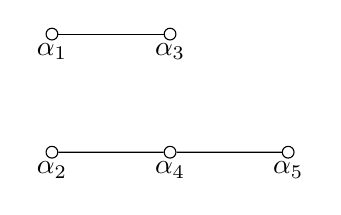
\begin{tikzpicture}[scale=1.5]
      \foreach \i in {1,2}
				\node[circle, draw, fill=white, inner sep=1.5pt] (\i) at (\i,0) {};
			\draw (1) -- (2);
      \node[below] at (1) {$\alpha_1$};
      \node[below] at (2) {$\alpha_3$};

      \foreach \i in {1,2,3}
				\node[circle, draw, fill=white, inner sep=1.5pt] (\i) at (\i,-1) {};
			\draw (1) -- (2) -- (3);
      \node[below] at (1) {$\alpha_2$};
      \node[below] at (2) {$\alpha_4$};
      \node[below] at (3) {$\alpha_5$};
    \end{tikzpicture}
  \end{minipage}
\end{figure}
\end{example}

\begin{definition}
  \label{defi:RootPairing.IsIrreducible}
  \lean{RootPairing.IsIrreducible}
  \leanok
  $R$-加群$M, N$に関するroot pairing $P$が次を満たすとき，$P$は\textbf{irreducible}であるという：
  \begin{enumerate}[label=(\roman*)]
    \item $M$は非自明である，すなわち$M \ne 0$.
    \item $N$は非自明である，すなわち$N \ne 0$.
    \item $M$の部分加群$q$が，任意のreflectionで不変(i.e., $s_i(q) \subseteq q$)で，$q \ne 0$であれば，$q = M$である．
    \item $N$の部分加群$q$が，任意のcoreflectionで不変で，$q \ne 0$であれば，$q = N$である．
  \end{enumerate}
\end{definition}

この定義が数学の文脈でのirreducible (Dynkin diagramが連結)であることを確かめる補題が次である：

\begin{lemma}
  \label{lem:RootPairing.Base.induction_on_cartanMatrix}
  \lean{RootPairing.Base.induction_on_cartanMatrix}
  \leanok
  root pairing $P$はreducedかつirreducibleであるとする．
  $p(i)$を添字$i$に対する命題とする．
  $i, j$を任意の添字とし，$p(i)$は真であるとする．
  さらに，$p$はDynkin diagramにおいて隣接で閉じている，すなわち次が成り立つとする：
  \begin{center}
    ($\ast$)\quad $p(k)$が真，かつCartan matrixの$(l, k)$成分が$0$でないならば，$p(l)$も真である．
  \end{center}
  このとき，$p(j)$は真である．
\end{lemma}

\begin{example}
  例~\ref{ex:A2xA3}はirreducibleでない．

  定義~\ref{defi:RootPairing.IsIrreducible}を満たさないことを確かめる．
  $A_2, A_3$にそれぞれ対応する部分加群は$M_1 := \operatorname{span}\{e_1, e_3\},\ M_2 := \operatorname{span}\{e_2, e_4, e_5\}$であり，$M_1 \oplus M_2 = M = \R^5$である．
  このとき，$s_1, s_3$は$M_1$内で作用し，$M_2$は固定する．
  また，$s_2, s_4, s_5$は$M_2$内で作用し，$M_1$は固定する．
  よって，$M_1, M_2$はそれぞれ任意のreflectionに対して不変である．

  補題~\ref{lem:RootPairing.Base.induction_on_cartanMatrix}の``気持ち''も理解しておく．
  命題$p(i)$として$i \in \{2, 4, 5\}$を考える．
  すると，これは条件($\ast$)を満たす．
  しかし，$p(1), p(3)$は偽であるから，$p$は任意の添字に対しては成り立たない．
  これは$A_2 \times A_3$がirreducibleでないからである．

  もしirreducibleなもので同じように$p(i)$として$i \in X$のような命題を考えたとき，$X$は添字全体になる．
\end{example}

\begin{theorem}
  \label{thm:diag_is_simeq_implies_FRG_is_simeq}
  $\Phi, \Phi'$をroot systemsとし，これらに対応するsimple root systemsをそれぞれ$\Delta, \Delta'$とする．
  また，$G_\Delta, G_{\Delta'}$をそれぞれ$\Delta, \Delta'$のCoxeter-Dynkin diagramとする．
  このとき，$G_\Delta \simeq G_{\Delta'}$なら$W_\Phi \simeq W_{\Phi'}$である．
\end{theorem}

\begin{theorem}
  \label{thm:coxeter_diag_classification}
  既約essential finite reflection groupのsimple root systemから定まるCoxeter-Dynkin diagramは，次の図においてcrystallographicであれば上9つ，そうでなければ下3つのいずれかである：
\end{theorem}


\newpage
\begin{proof}
  まず，これらのdiagramsはfinite reflection groupsに対応することを示す．
  $\{e_1, \ldots, e_r\}$を$\R^r$の標準基底とする．

  \vspace{10pt}
  \noindent
  \underline{$A_n$型}

  \begin{gather}
    V := \set{\sum_{i=1}^{n+1} a_i e_i}{\sum_{i=1}^{n+1} a_i = 0} \subseteq \R^{n+1},\\
    \begin{split}
      \Phi &:= \set{v \in V}{\inner{v}{v} = 2} \cap \bigoplus_{i=1}^{n+1} \Z e_i\\
      &= \set{e_i - e_j}{1 \le i \ne j \le n+1},
    \end{split}\\
    \Delta := \set{\alpha_i := e_i - e_{i+1}}{1 \le i \le n},\\
    W \simeq \mathfrak{S}_{n+1},\ s_{\alpha_i} \mapsto (i\ j).
  \end{gather}
  とすれば，$i \ne j$のとき
  \begin{equation}
    (s_{\alpha_i} s_{\alpha_j}\textrm{の位数})
    = ((i\ i+1)(j\ j+1)\textrm{の位数})
    = \begin{cases}
      2 & (|i - j| \ge 2)\\
      3 & (|i - j| = 1)
    \end{cases}
  \end{equation}
  となるから$A_n$型のdiagramが得られる．

  \vspace{10pt}
  \noindent
  \underline{$B_n$型}

  $|\Phi| = 2n^2$で，長さの$2$乗が$1$のものが$2n$個，$2$のものが$2n(n-1)$個ある．
  \begin{gather}
    V := \R^n,\\
    \begin{split}
      \Phi &:= \set{v \in V}{\inner{v}{v} \in \{1, 2\}} \cap \bigoplus_{i=1}^{n} \Z e_i\\
      &= \set{\pm e_i}{1 \le i \le n} \cup \set{\pm (e_i + e_j)}{1 \le i < j \le n},
    \end{split}\\
    \Delta := \set{\alpha_i := e_i - e_{i+1},\ \alpha_n := e_n}{1 \le i \le n-1},\\
    W \simeq \mathfrak{S}_n \ltimes (\Z/2\Z)^n,\ \textrm{$\mathfrak{S}_n$は$s_{\alpha_i} \mapsto (i\ j)$で，$(\Z/2\Z)^n$は$e_i \mapsto -e_i$で作用．}
  \end{gather}

  \vspace{10pt}
  \noindent
  \underline{$C_n$型}

  $C_n$型は$B_n$型の``双対''である．
  \begin{gather}
    V := \R^n,\\
    \begin{split}
      \Phi &:= \set{v \in V}{\inner{v}{v} \in \{2, 4\}} \cap \bigoplus_{i=1}^{n} \Z e_i\\
      &= \set{\pm 2e_i}{1 \le i \le n} \cup \set{\pm (e_i + e_j)}{1 \le i < j \le n},
    \end{split}\\
    \Delta := \set{\alpha_i := e_i - e_{i+1},\ \alpha_n := 2e_n}{1 \le i \le n-1},\\
    W \simeq \mathfrak{S}_n \ltimes (\Z/2\Z)^n,\ \textrm{作用は$B_n$型と同じ．}
  \end{gather}

  \vspace{10pt}
  \noindent
  \underline{$D_n$型}
  \begin{gather}
    V := \R^n,\\
    \begin{split}
      \Phi &:= \set{v \in V}{\inner{v}{v} = 2} \cap \bigoplus_{i=1}^{n} \Z e_i\\
      &= \set{\pm (e_i + e_j)}{1 \le i < j \le n},
    \end{split}\\
    \Delta := \set{\alpha_i = e_i - e_{i+1},\ \alpha_n = e_{n-1} + e_n}{1 \le i \le n-1},\\
    W \simeq \mathfrak{S}_n \ltimes (\Z/2\Z)^{n-1},\ \textrm{$\mathfrak{S}_n$は$s_{\alpha_i} \mapsto (i\ j)$で，$(\Z/2\Z)^{n-1}$は偶数個の符号変換$e_i \mapsto -e_i$で作用．}
  \end{gather}

  \vspace{10pt}
  \noindent
  \underline{$G_2$型}
  \begin{gather}
    V := \set{\sum_{i=1}^{3} a_i e_i}{\sum_{i=1}^{3} a_i = 0} \subseteq \R^3,\\
    \begin{split}
      \Phi &:= \set{v \in V}{\inner{v}{v} = \{2, 6\}} \cap \bigoplus_{i=1}^{3} \Z e_i\\
      &= \set{\pm(e_i - e_j)}{1 \le i < j \le 3} \cup \set{\pm(2e_i - e_j - e_k)}{\{i, j, k\} = \{1, 2, 3\}},
    \end{split}\\
    \Delta := \{\alpha_1 := e_1 - e_2,\ \alpha_2 = -2e_1 + e_2 + e_3\},\\
    W \simeq \mathcal{D}_6\ (\textrm{位数12の二面体群}).
  \end{gather}

  \vspace{10pt}
  \noindent
  \underline{$F_4$型}

  補助的に格子$\Lambda \subseteq V$を導入する．$|\Phi| = 48$で，長さの$2$乗が$1$のものと$2$のものがそれぞれ$24$個ある．
  \begin{gather}
    V := \R^4,\\
    \Lambda := \bigoplus_{i=1}^{4} \Z e_i + \Z \left( \frac{1}{2} \sum_{i=1}^{4} e_i \right),\\
    \begin{split}
      \Phi &:= \set{v \in \Lambda}{\inner{v}{v} = \{1, 2\}}\\
      &= \set{\pm (e_i + e_j)}{1 \le i < j \le 4} \cup \set{\pm e_i}{1 \le i \le 4} \cup \{\frac{1}{2}(\pm e_1 \pm e_2 \pm e_3 \pm e_4)\},
    \end{split}\\
    \Delta := \{\alpha_1 := e_2-e_3,\ \alpha_2 := e_3-e_4,\ \alpha_3 := e_4,\ \alpha_4 := \frac{1}{2}(e_1-e_2-e_3-e_4)\}.
  \end{gather}

  \vspace{10pt}
  \noindent
  \underline{$E_8$型}

  補助的に格子$\Lambda \subseteq V$を導入する．
  $|\Phi| = 4 \cdot 28 + 2^8 / 2 = 112 + 128 = 240$である．
  \begin{gather}
    V := \R^8,\\
    \Lambda := \set{\sum_{i=1}^{8} c_i e_i}{c_i \in \Z,\ \sum_{i=1}^{8} e_i \in 2\Z} + \Z \left(\frac{1}{2} \sum_{i=1}^{8} e_i\right),\\
    \begin{split}
      \Phi &:= \set{v \in \Lambda}{\inner{v}{v} = 2}\\
      &= \set{\pm (e_i + e_j)}{1 \le i < j \le 8} \cup \set{\frac{1}{2} \sum_{i=1}^{8} \pm e_i}{\textrm{マイナスが偶数個}},
    \end{split}\\
    \Delta := \{\alpha_1 := \frac{1}{2} (e_1 - e_2 - \cdots - e_7 + e_8),\ \alpha_2 := e_1 + e+2,\ \alpha_i = e_{i-1} - e_{i-2}\ (3 \le i \le 8)\}.
  \end{gather}

  \vspace{10pt}
  \noindent
  \underline{$E_7$型}

  Coxeter-Dynkin diagramが$E_8$型の部分グラフであることに注意する．
  $E_8$型の$\alpha_i$を用いる．
  $|\Phi| = 4 \cdot 15 + 2 + 2 \cdot (6 + 20 + 6) = 126$である．
  \begin{gather}
    V := \R\{\alpha_1, \ldots, \alpha_7\} \subseteq \R^8,\\
    \begin{split}
      \Phi &:= \Phi_{E_8} \cap V\\
      &= \set{\pm (e_i + e_j)}{1 \le i < j \le 6} \cup \{\pm (e_7 - e_8)\} \cup \set{\pm \frac{1}{2} \left(e_7 - e_8 + \sum_{i=1}^{6} \pm e_i\right)}{\textrm{$\sum$の中のマイナスは奇数個}},
    \end{split}\\
    \Delta := \{\alpha_1, \ldots, \alpha_7\}.
  \end{gather}

  \vspace{10pt}
  \noindent
  \underline{$E_6$型}

  Coxeter-Dynkin diagramが$E_8$型の部分グラフであることに注意する．
  $E_8$型の$\alpha_i$を用いる．
  \begin{gather}
    V := \R\{\alpha_1, \alpha_6\} \subseteq \R^n,\\
    \begin{split}
      \Phi &:= \Phi_{E_8} \cap V\\
      &= \set{\pm (e_i - e_j)}{1 \le i < j \le 5} \cup \set{\pm \frac{1}{2}\left(e_8 - e_7 - e_6 + \sum_{i=1}^{5} \pm e_i\right)}{\textrm{$\sum$の中のマイナスは奇数個}},
    \end{split}\\
    \Delta := \{\alpha_1, \ldots, \alpha_6\}.
  \end{gather}

\end{proof}

\begin{proposition}
  $W_1, W_2$をessential finite reflection groupsとし，$G_{\Delta_1}, G_{\Delta_2}$をそれぞれ対応するCoxeter-Dynkin diagramとする．
  このとき，$W_1 \times W_2$はessential finite reflection groupであり，そのCoxeter-Dynkin diagramは$G_{\Delta_1} \sqcup G_{\Delta_2}$である．
\end{proposition}

よって，任意のessential finite reflection groupから定まるCoxeter-Dynkin diagramは，図~\ref{fig:coxeter_diag_classification}の組み合わせで表される．
